% ============================================================
%  IEEE_QUANTUM_AUDIT_PAPER_v2.tex
%  An Independent Statistical Audit of Adaptive Quantum Kernel
%  Selection for Clinical Cancer Benchmarks: Multi-Seed Robustness,
%  Familywise Error Control, and Cross-Dataset Generalization
%  IEEE Transactions format — double column
%  Author: Muhammad Wajahat, Member, IEEE
% ============================================================
\documentclass[journal,twocolumn]{IEEEtran}

% ---- Packages ----
\usepackage{amsmath,amssymb,amsfonts,amsthm}
\usepackage{booktabs,tabularx,multirow,makecell,array,longtable}
\usepackage{graphicx,xcolor}
\usepackage{cite}
\usepackage{microtype}
\usepackage{url}
\usepackage{bm}
\usepackage{tikz}
\usetikzlibrary{shapes.geometric,arrows.meta,positioning,calc,fit,backgrounds,decorations.pathreplacing,matrix,patterns}
\usepackage{pgfplots}
\pgfplotsset{compat=1.18}
\usepackage{pgfplotstable}
\usepackage{hyperref}

% ---- Colors ----
\definecolor{auditblue}{RGB}{20,50,110}
\definecolor{auditgreen}{RGB}{20,95,50}
\definecolor{auditred}{RGB}{145,25,25}
\definecolor{auditgray}{RGB}{245,247,250}
\definecolor{quantumteal}{RGB}{0,110,130}
\definecolor{classicalorange}{RGB}{180,80,0}

% ---- Theorems ----
\newtheorem{definition}{Definition}
\newtheorem{remark}{Remark}

% ---- Hyperref ----
\hypersetup{
  colorlinks=true,
  linkcolor=auditblue,
  citecolor=auditgreen,
  urlcolor=quantumteal
}

% ---- Column types for tables ----
\newcolumntype{C}[1]{>{\centering\arraybackslash}p{#1}}
\newcolumntype{L}[1]{>{\raggedright\arraybackslash}p{#1}}

% ============================================================
\begin{document}
% ============================================================

\title{An Independent Statistical Audit of Adaptive Quantum Kernel Selection for Clinical Cancer Benchmarks: Multi-Seed Robustness, Familywise Error Control, and Cross-Dataset Generalization}

\author{Muhammad~Wajahat,~\IEEEmembership{Member,~IEEE}%
\thanks{Manuscript submitted October 2026.}%
\thanks{The author is with the Department of Computer Science, National Biomedical Computational Center, Islamabad, Pakistan (e-mail: wajahat.cs@nbcc.edu.pk).}}

\maketitle

% ============================================================
\begin{abstract}
Quantum machine learning (QML) frameworks have attracted substantial clinical interest as potential tools for oncology decision support, with recent work claiming that an adaptive quantum kernel stacking ensemble surpasses classical support vector machines across multiple benchmarks. This paper presents a rigorous, code-level statistical audit of one such framework---Daga et al.\ (2026)---applied to the Wisconsin Diagnostic Breast Cancer (WDBC) dataset ($N=569$), independently replicated on the Wisconsin Breast Cancer Original (WBCO) dataset ($N=683$),  Our audit identifies five fundamental methodological vulnerabilities in the published literature: single-seed evaluation, absence of familywise error rate (FWER) control, un-tuned classical baselines, hardcoded rather than adaptive kernel selection, and a depolarizing noise implementation error causing unphysical trace collapse. Empirically, Classical RBF-SVM equals or outperforms the claimed quantum stacking ensemble in \textbf{20 out of 20 seed comparisons} across both diagnostic datasets (10 on WDBC, 10 on WBCO, zero losses). A 32-hypothesis Holm--Bonferroni bootstrap audit identifies zero quantum-superior findings on WDBC after FWER control; on WBCO, one quantum-superior metric (QKNN-Angle Recall, $p < 0.0001$) survives, with no ensemble-level statistical advantage confirmed. Fold-local two one-sided tests (TOST) confirm practical equivalence within $\pm 1\%$ on both datasets ($p = 0.0385$ for WDBC, $p = 0.0004$ for WBCO). Exhaustive nested model selection reveals that QSVM-Angle, excluded from the published ensemble quartet, is selected in 10 of 10 folds on both datasets, while the paper's claimed quartet is selected in 0 of 10 folds on WDBC and at most 1 of 10 on WBCO. These comprehensive findings demonstrate that the claimed quantum advantage is not statistically supported across either clinical cytology benchmark.
\end{abstract}

\begin{IEEEkeywords}
Quantum machine learning, support vector machine, quantum kernel, NISQ devices, cancer diagnosis, estrogen receptor, statistical audit, Holm--Bonferroni correction, TOST, model selection, McNemar test, depolarizing noise.
\end{IEEEkeywords}

% ============================================================
\section{Introduction}
% ============================================================

\IEEEPARstart{B}{reast} cancer is among the most prevalent malignancies worldwide, accounting for more than 2.3 million new cases and 685,000 deaths annually \cite{globocan2020}. In clinical oncology, computational decision support primarily targets \textit{diagnostic classification}, where an undiagnosed breast lesion is classified as benign or malignant based on cytological or histopathological morphology \cite{bray2018global,mangasarian1995breast}. In both settings, decision accuracy carries severe asymmetric clinical costs: false negatives delay critical life-saving interventions, while false positives trigger unnecessary invasive procedures, physical morbidity, and emotional distress.

In parallel with advances in classical supervised learning, the emergence of noisy intermediate-scale quantum (NISQ) devices \cite{preskill2018quantum} has stimulated intense investigation into \textit{quantum machine learning} (QML) for biomedical data \cite{biamonte2017quantum}. Quantum kernel methods, in particular, evaluate the inner product between quantum states mapped into a high-dimensional Hilbert space, $\mathcal{H}$, via parameterized quantum circuits \cite{havlicek2019supervised,schuld2021supervised}. By mapping classical feature vectors $\mathbf{x} \in \mathbb{R}^D$ into quantum statevectors $|\psi(\mathbf{x})\rangle \in \mathcal{H}$, quantum kernels offer an elegant interface with classical support vector machine (SVM) optimization algorithms \cite{rebentrost2014quantum}. Theoretical results demonstrate that certain quantum feature maps are classically hard to evaluate, establishing potential computational separations for structured synthetic distributions \cite{liu2021rigorous}.

Despite these theoretical foundations, the empirical evidence for practical quantum advantage on real-world medical datasets has remained contentious and methodologically fragile \cite{krol2022variational,cerezo2021variational}. Daga et al.\ (2026) \cite{daga2026adaptive} represent a prominent recent claim in this domain, introducing an ``adaptive quantum kernel selection'' stacking ensemble framework. The authors report that combining quantum support vector machines (QSVM) and quantum $k$-nearest neighbors (QKNN) equipped with Angle, ZZ (IQP-style), and Amplitude feature maps yields superior classification accuracy and simulated noise resilience compared to a classical Radial Basis Function (RBF) SVM baseline on clinical benchmarks, including the Wisconsin Diagnostic Breast Cancer (WDBC) dataset. Similar claims of quantum supremacy on small medical cohorts have proliferated across recent literature \cite{li2015experimental,altares2021automatic}, frequently evaluated on single cross-validation splits without familywise error rate (FWER) control.

This paper conducts a rigorous, multi-tiered independent audit of the Daga et al.\ framework. Our investigation is motivated by the recognized need for scientific reproducibility in QML \cite{krol2022variational} and the strict evidential standards required before deploying algorithmic models into clinical workflows. We identify five critical methodological deficiencies in the original work (Section~\ref{sec:problem}), construct a five-tier statistical audit protocol targeting each vulnerability, apply this protocol to WDBC ($N=569$), and independently replicate it on the Wisconsin Breast Cancer Original (WBCO, $N=683$) dataset.

\subsection{The NISQ Reality and Simulation Fidelity}

Current NISQ processors operate under severe decoherence, cross-talk, and gate infidelities that constrain circuit depth and qubit capacity \cite{preskill2018quantum}. Consequently, QML algorithms are predominantly simulated on classical computing clusters. In such simulations, accurately modeling noise channels is paramount for evaluating real-world viability. The standard single-parameter depolarizing noise channel $\mathcal{E}(\rho) = (1-p)\rho + \frac{p}{2^n}\mathbf{I}$ represents isotropic decoherence \cite{nielsen2010quantum}. However, implementing this channel physically requires the density matrix formalism with trace preservation ($\text{Tr}[\mathcal{E}(\rho)]=1$). As shown in Section~\ref{sec:results}, the original code implements an unnormalized statevector damping approximation that results in severe trace collapse, rendering published noise robustness metrics unphysical.

\subsection{Algorithmic Adaptivity vs.\ Hardcoded Ensembles}

A central claim of the audited framework is ``adaptive'' kernel selection. In practice, our code-level audit reveals that no algorithmic selection mechanism is implemented: the ensemble is fixed a priori to a four-model quartet (QSVM-ZZ, QSVM-Amplitude, QKNN-ZZ, QKNN-Amplitude). Crucially, exhaustive nested cross-validation reveals that the single highest-performing quantum model---QSVM-Angle---is consistently selected across 10 of 10 folds on both WDBC and WBCO, yet it is excluded from the paper's ensemble without theoretical or empirical justification.

\subsection{Paper Organization}

The remainder of this paper is structured as follows. Section~\ref{sec:litreview} reviews related work and presents a systematic literature comparison. Section~\ref{sec:problem} formulates the problem statement, details five methodological deficiencies, and enumerates seven contributions. Section~\ref{sec:methodology} describes the audited architecture, mathematical kernel definitions, statistical testing protocols, and noise auditing equations. Section~\ref{sec:results} presents comprehensive empirical results across ten subsections, including multi-seed evaluations, Holm--Bonferroni audits, TOST equivalence tests, model selection audits, noise verifications, and cross-dataset generalization assessments. Section~\ref{sec:threats} examines threats to validity, and Section~\ref{sec:conclusion} concludes.

% ============================================================
\section{Literature Review and Related Work}
\label{sec:litreview}
% ============================================================

\subsection{Quantum Kernel Methods in Supervised Learning}

Quantum kernel methods represent a leading paradigm for NISQ-era quantum computing \cite{havlicek2019supervised,schuld2021supervised}. Havl{\'i}{\v c}ek et al.\ \cite{havlicek2019supervised} experimentally demonstrated quantum kernel estimation on superconducting quantum hardware, introducing the entangling ZZ feature map derived from instantaneous quantum polynomial (IQP) circuits. Schuld and Killoran \cite{schuld2021supervised} provided a unified geometric framework proving that quantum kernel machines operate as linear classifiers within a reproducing kernel Hilbert space (RKHS) associated with the quantum state representation. Liu et al.\ \cite{liu2021rigorous} proved that quantum kernels can achieve a provable superpolynomial speedup over classical learners on engineered discrete log problems. However, on classically tractable, continuous tabular distributions, classical kernel methods often match or exceed quantum kernels in expressive capacity \cite{tang2019quantum}.

\subsection{QML in Medical and Biological Data}

Medical diagnostic classification has emerged as an attractive application domain for QML algorithms \cite{li2015experimental,altares2021automatic}. Li et al.\ \cite{li2015experimental} implemented a proof-of-concept QSVM on an optical quantum processor for breast cancer detection using low-dimensional feature projections. Altares-L{\'o}pez et al.\ \cite{altares2021automatic} proposed automated feature map design heuristics on UCI datasets. However, these foundational works were evaluated on small sample sizes ($N < 200$) without multi-seed partitioning, cross-dataset replication, or FWER adjustments. Table~\ref{tab:litcomp} summarizes the methodological dimensions of representative QML studies alongside the audited framework of Daga et al.\ (2026).

\subsection{Statistical Auditing and Multiple Testing in Machine Learning}

The necessity for rigorous statistical testing in comparative ML evaluation is widely recognized \cite{demsar2006statistical,efron1994introduction}. Testing multiple models across diverse clinical performance metrics generates a severe multiple comparisons problem. Under familywise error rate (FWER) control, the probability of incurring at least one type~I error across $m$ simultaneous hypotheses is constrained to $\alpha$. The Holm--Bonferroni step-down procedure \cite{holm1979simple} provides strong FWER control without requiring independence assumptions, making it substantially more powerful than classical Bonferroni adjustment. Complementarily, two one-sided tests (TOST) \cite{wellek2010testing} evaluate practical equivalence within an indifference margin $\pm \epsilon$, distinguishing meaningful algorithmic discrepancies from negligible numerical fluctuations.

\subsection{Out-of-Fold Stacking and Meta-Learning}

Stacked generalization (stacking) combines heterogeneous base learners through a secondary meta-model trained on out-of-fold (OOF) cross-validation predictions \cite{wolpert1992stacked}. While stacking can enhance predictive stability, its performance is sensitive to base model diversity, meta-learner regularizers, and class imbalance. In the audited framework, a logistic regression meta-learner with balanced class weights is applied to OOF probability vectors. Our audit investigates whether this stacking architecture confers an authentic clinical advantage over individual quantum kernels and tuned classical baselines.

\begin{table*}[!t]
\caption{Comprehensive Literature Comparison: Methodological Dimensions Across Representative QML Papers}
\label{tab:litcomp}
\centering
\footnotesize
\renewcommand{\arraystretch}{1.2}
\begin{tabularx}{\textwidth}{>{\raggedright\arraybackslash\bfseries}p{3.2cm} *{6}{>{\centering\arraybackslash}X}}
\toprule
Dimension & Havl{\'i}{\v c}ek et al.\ (2019) & Schuld \& Killoran (2021) & Liu et al.\ (2021) & Altares-L{\'o}pez et al.\ (2021) & Li et al.\ (2015) & Daga et al.\ (2026) [Audited] \\
\midrule
Dataset(s) & Synthetic & Synthetic & Structured & Iris, MNIST & Breast cancer & WDBC, IoT, GeneEx \\
Multi-seed evaluation & No & No & No & No & No & No (seed=42 only) \\
FWER-controlled testing & N/A & N/A & Theorem-based & No & No & No \\
Classical baseline tuning & N/A & N/A & N/A & Basic & Basic & Untuned ($C=1$, default) \\
Noise model correctness & N/A & N/A & N/A & N/A & N/A & Error: trace collapse \\
Model selection verification & N/A & N/A & Proved & No & No & Hardcoded, not adaptive \\
Cross-dataset replication & No & No & No & No & No & No (audit adds WBCO) \\
\bottomrule
\end{tabularx}
\end{table*}

% ============================================================
\section{Problem Statement and Contributions}
\label{sec:problem}
% ============================================================

\subsection{Problem Statement}

In oncology decision support, misclassification carries severe, irreversible clinical costs. Delayed detection of an aggressive malignancy directly correlates with stage migration and patient mortality. Conversely, a false-positive finding triggers invasive biopsies, patient trauma, and costly medical overhead. Consequently, computational claims of state-of-the-art diagnostic accuracy or noise resilience require flawless statistical grounding.

Daga et al.\ (2026) \cite{daga2026adaptive} report that an adaptive quantum kernel stacking framework achieves superior diagnostic accuracy and noise robustness over classical SVM baselines on WDBC and other benchmarks. However, our code-level audit reveals five critical methodological vulnerabilities that undermine the scientific validity of these conclusions:

\begin{enumerate}
    \item \textbf{Single-Seed Partition Vulnerability.} All published performance metrics rely entirely on a single cross-validation split (seed=42). A single seed cannot separate systematic algorithmic superiority from random partition favorability, introducing severe variance risk.
    \item \textbf{Absence of Multiple Testing (FWER) Control.} Evaluating 8 candidate models across 4 primary clinical metrics produces 32 simultaneous statistical hypotheses. At an uncorrected significance level of $\alpha = 0.05$, the probability of encountering at least one false positive exceeds $1 - (0.95)^{32} \approx 80.6\%$.
    \item \textbf{Artificially Untuned Classical Baseline.} The classical RBF-SVM baseline was evaluated using default Scikit-Learn hyperparameters ($C=1.0$, $\gamma=\text{'scale'}$) without grid search, creating an unfairly constrained comparison target.
    \item \textbf{Hardcoded Pseudo-Adaptivity.} While titled ``adaptive quantum kernel selection,'' the software pipeline implements a fixed, hardcoded 4-model quartet with zero algorithmic selection logic, while omitting the highest-performing base model (QSVM-Angle).
    \item \textbf{Noise Model Trace Collapse.} The depolarizing noise implementation evaluates statevectors rather than normalized density matrices, causing unphysical trace decay ($K_{ii} \in [0.1982, 0.2310]$ in released code vs.\ $K_{ii} \in [0.0041, 0.0162]$ under physical density matrix normalization), inflating perceived quantum coherence by $\approx 15\times$.
\end{enumerate}

\begin{remark}
This audit addresses four core scientific questions: (i)~Does the quantum ensemble's empirical advantage survive multi-seed evaluation? (ii)~Do quantum-superior findings survive rigorous FWER correction? (iii)~Is the claimed adaptivity verifiable in code? (iv)~Does the pipeline generalize across an independent diagnostic clinical cohort (WBCO)?
\end{remark}

\subsection{Contributions}

This paper makes six concrete contributions:
\begin{enumerate}
    \item \textbf{Exact Baseline Reproduction.} We replicate the published WDBC results down to machine precision at seed=42 (confusion matrices match exactly: TN=201, FP=11, FN=6, TP=351 for RBF; TN=200, FP=12, FN=8, TP=349 for Stacking), confirming complete pipeline execution fidelity.
    \item \textbf{Multi-Seed Robustness Audit across 20 Seeds.} Over 10 random seeds on WDBC and 10 on WBCO, Classical RBF-SVM equals or outperforms OOF Stacking in \textbf{20 out of 20 evaluations} (10 wins on WDBC; 7 wins and 3 ties on WBCO; 0 losses).
    \item \textbf{32-Hypothesis Holm--Bonferroni Audit.} Bootstrap testing with Holm step-down correction reveals zero quantum-superior findings on WDBC after FWER control. On WBCO, exactly one quantum-superior metric survives (QKNN-Angle Recall, $p < 0.0001$), with zero ensemble-level advantage confirmed.
    \item \textbf{Fold-Local TOST Equivalence Audit.} Two one-sided tests confirm practical equivalence ($\pm 1\%$ margin) between fold-local and global preprocessing on both WDBC ($p = 0.0385$) and WBCO ($p = 0.0004$), ruling out data leakage as a confounding factor.
    \item \textbf{Nested Model Selection Discrepancy.} Nested CV demonstrates that QSVM-Angle is selected in 10 of 10 folds across both datasets, whereas the paper's claimed quartet is selected in 0 of 10 folds on WDBC and at most 1 of 10 on WBCO.
    \item \textbf{Cross-Dataset WBCO Replication.} Independent replication on WBCO ($N=683$) confirms 2 of 4 core audit findings fully and 2 partially.
\end{enumerate}

% ============================================================
\section{Audited Architecture and Methodology}
\label{sec:methodology}
% ============================================================

Fig.~\ref{fig:pipeline} illustrates the comprehensive architectural and statistical auditing workflow across both clinical cohorts.

\subsection{Clinical Cohorts and Preprocessing Pipeline}

The audit evaluates two clinical diagnostic cohorts:
\begin{itemize}
    \item \textbf{WDBC Cohort ($N=569$):} Diagnostic cytological cohort comprising $D=30$ continuous nuclear morphometry features derived from digitized fine needle aspirates (FNA). Malignant: 212 ($37.26\%$), Benign: 357 ($62.74\%$).
    \item \textbf{WBCO Extension ($N=683$):} Diagnostic histopathological cohort comprising $D=9$ cytological features scored on an integer scale $[1, 10]$ (16 instances with missing values excluded). Malignant: 239 ($34.99\%$), Benign: 444 ($65.01\%$).
\end{itemize}

\begin{definition}[Preprocessing Pipeline]
For raw feature matrix $\mathbf{X} \in \mathbb{R}^{N \times D}$, the three-stage normalization pipeline is:
\begin{align}
    \mathbf{X}^{(1)} &= \frac{\mathbf{X} - \boldsymbol{\mu}}{\boldsymbol{\sigma}}, \label{eq:standardize} \\
    \mathbf{X}^{(2)} &= \text{PCA}_K(\mathbf{X}^{(1)}), \label{eq:pca} \\
    \mathbf{X}^{(3)} &= \frac{\mathbf{X}^{(2)} - \mathbf{X}^{(2)}_{\min}}{\mathbf{X}^{(2)}_{\max} - \mathbf{X}^{(2)}_{\min}} \cdot \pi, \label{eq:minmax}
\end{align}
where $\boldsymbol{\mu}, \boldsymbol{\sigma}$ denote training-set feature statistics, $K=8$ principal components are extracted, and MinMax scaling maps features into the gate domain $[0, \pi]$.
\end{definition}

The cumulative variance retention ratio $\text{VR}(K)$ is:
\begin{equation}
    \text{VR}(K) = \frac{\sum_{k=1}^{K} \lambda_k}{\sum_{j=1}^{D} \lambda_j},
    \label{eq:pca_var}
\end{equation}
where $\lambda_k$ are covariance eigenvalues. At $K=8$, WDBC retains $92.598\%$ variance ($D=30$), and WBCO retains $99.018\%$ ($D=9$), both comfortably exceeding standard biomedical variance retention thresholds ($\ge 90\%$).

\subsection{Quantum Kernel Formulations}

\begin{definition}[Quantum Kernel Inner Product]
For state $|\psi(\mathbf{x})\rangle = \mathcal{U}(\mathbf{x})|0\rangle^{\otimes n}$ generated by unitary $\mathcal{U}$, the quantum kernel is defined as:
\begin{equation}
    K(\mathbf{x}_i, \mathbf{x}_j) = |\langle\psi(\mathbf{x}_i)|\psi(\mathbf{x}_j)\rangle|^2 = \text{Tr}[\rho(\mathbf{x}_i)\rho(\mathbf{x}_j)],
    \label{eq:qkernel}
\end{equation}
where $\rho(\mathbf{x}) = |\psi(\mathbf{x})\rangle\langle\psi(\mathbf{x})|$.
\end{definition}

\textbf{Angle Embedding Kernel.} The $n$-qubit Angle embedding applies single-qubit $R_X(x_k)$ Pauli rotations on each wire (Fig.~\ref{fig:circuit}):
\begin{equation}
    K_{\text{Angle}}(\mathbf{x}_i, \mathbf{x}_j) = \prod_{k=1}^{n} \cos^2\!\left(\frac{x_{ik} - x_{jk}}{2}\right).
    \label{eq:angle_kernel}
\end{equation}
This product kernel permits exact closed-form evaluation without circuit simulation overhead ($n=8$ qubits).

\textbf{ZZ Feature Map Kernel (IQP-Style).} The ZZ entangling feature map applies Hadamards and parameterized two-qubit Ising interactions:
\begin{equation}
    \mathcal{U}_{ZZ}(\mathbf{x}) = \prod_{(j,k)\in S} \exp\!\left(-i\frac{(\pi - x_j)(\pi - x_k)}{2} Z_j \otimes Z_k\right) \cdot H^{\otimes n},
    \label{eq:zz_circuit}
\end{equation}
where $S$ denotes nearest-neighbor qubit pairs ($n=8$ qubits).

\textbf{Amplitude Embedding Kernel.} Amplitude embedding encodes normalized feature vectors directly into quantum state amplitudes using $n=3$ qubits for 8-dimensional inputs ($2^3 = 8$):
\begin{equation}
    K_{\text{Amp}}(\mathbf{x}_i, \mathbf{x}_j) = \left(\frac{\mathbf{x}_i^\top \mathbf{x}_j}{\|\mathbf{x}_i\|\|\mathbf{x}_j\|}\right)^2,
    \label{eq:amp_kernel}
\end{equation}
corresponding to squared cosine similarity.

% ============================================================
% FIGURE 1: Redesigned Clean TikZ Architecture Diagram
% ============================================================
\begin{figure*}[!t]
\centering
\begin{tikzpicture}[
  font=\scriptsize,
  box/.style={draw, rounded corners=3pt, align=center, inner sep=3pt, line width=0.5pt},
  databox/.style={box, fill=auditgray, draw=auditblue!80, text width=2.1cm, minimum height=0.85cm},
  prepbox/.style={box, fill=auditblue!10, draw=auditblue, text width=2.1cm, minimum height=3.6cm},
  cbox/.style={box, fill=classicalorange!15, draw=classicalorange, text width=2.4cm, minimum height=0.65cm},
  qbox/.style={box, fill=quantumteal!15, draw=quantumteal, text width=2.4cm, minimum height=0.65cm},
  sbox/.style={box, fill=auditblue!15, draw=auditblue, font=\scriptsize\bfseries, text width=2.3cm, minimum height=0.85cm},
  vbox/.style={box, fill=auditgray!80, draw=gray, font=\scriptsize\bfseries, text width=2.3cm, minimum height=0.75cm},
  auditbox/.style={box, fill=auditred!10, draw=auditred, text width=2.5cm, minimum height=0.6cm},
  outbox/.style={box, fill=auditgreen!15, draw=auditgreen, font=\scriptsize, text width=2.2cm, minimum height=4.2cm},
  arr/.style={-{Stealth[length=1.8mm]}, thick, draw=gray!80},
  carr/.style={-{Stealth[length=1.8mm]}, thick, draw=classicalorange, dashed},
  qarr/.style={-{Stealth[length=1.8mm]}, thick, draw=quantumteal},
  aarr/.style={-{Stealth[length=1.8mm]}, thick, draw=auditred}
]

% Column Headers
\node[font=\tiny\bfseries, text=auditblue] at (1.2, 2.7) {1. Clinical Cohorts};
\node[font=\tiny\bfseries, text=auditblue] at (4.1, 2.7) {2. Preprocessing};
\node[font=\tiny\bfseries, text=quantumteal] at (7.3, 2.7) {3. Feature Maps \& Models};
\node[font=\tiny\bfseries, text=auditblue] at (10.5, 2.7) {4. Ensembles};
\node[font=\tiny\bfseries, text=auditred] at (13.7, 2.7) {5. Multi-Tier Audit};
\node[font=\tiny\bfseries, text=auditgreen] at (16.9, 2.7) {6. Audited Outcomes};

% STAGE 1: Clinical Cohorts
\node[databox] (wdbc) at (1.2, 1.0) {\textbf{WDBC Cohort}\\$N=569, D=30$\\{\tiny (37.3\% Malignant)}};
\node[databox] (wbco) at (1.2, -1.0) {\textbf{WBCO Extension}\\$N=683, D=9$\\{\tiny (35.0\% Malignant)}};

% STAGE 2: Preprocessing
\node[prepbox] (prep) at (4.1, 0.0) {\textbf{Preprocessing}\\[4pt]
\textbullet~$z$-Score Norm.\\[2pt]
\textbullet~PCA ($K=8$ Dim)\\
{\tiny WDBC: 92.6\% Var}\\
{\tiny WBCO: 99.0\% Var}\\
\textbullet~MinMax $[0, \pi]$\\[2pt]
{\tiny (Fixed 8-Qubit Budget)}};

% STAGE 3: Models
\node[cbox] (rbf) at (7.3, 1.8) {\textbf{Classical RBF-SVM}\\Direct PCA ($C=1,\gamma=\text{'scale'}$)\phantom{X}};
\node[qbox] (angle) at (7.3, 0.6) {\textbf{Angle Map (8-Qubit)}\\QSVM-Ang \& QKNN-Ang};
\node[qbox] (zz) at (7.3, -0.6) {\textbf{ZZ / IQP Map (8-Qubit)}\\QSVM-ZZ \& QKNN-ZZ};
\node[qbox] (amp) at (7.3, -1.8) {\textbf{Amp Map (3-Qubit)}\\QSVM-Amp \& QKNN-Amp};

% STAGE 4: Ensembles
\node[vbox] (voting) at (10.5, 1.0) {\textbf{Hard Majority Vote}\\3 Quantum Models\\(ZZ, Amp, Angle)};
\node[sbox] (stack) at (10.5, -1.0) {\textbf{OOF Stacking Ens.}\\5-Fold Meta-CV\\Logistic Regression\\(Amp, ZZ, Angle)};

% STAGE 5: Audit Suite
\node[auditbox] (aud1) at (13.7, 2.0) {\textbf{1. Multi-Seed Robustness}\\10 Seeds (20 Runs)};
\node[auditbox] (aud2) at (13.7, 1.0) {\textbf{2. Holm FWER Test}\\32 Hypotheses ($\alpha=0.05$)};
\node[auditbox] (aud3) at (13.7, 0.0) {\textbf{3. Fold-Local TOST}\\$\pm 1\%$ Equivalence Margin};
\node[auditbox] (aud4) at (13.7, -1.0) {\textbf{4. Nested Selection}\\Exhaustive $C(6,4)$ Search};
\node[auditbox] (aud5) at (13.7, -2.0) {\textbf{5. Noise Verification}\\Density Matrix Audit};

% STAGE 6: Outcomes
\node[outbox] (verdict) at (16.9, 0.0) {\textbf{Audited Diagnostic}\\[1pt]
\textbf{\& Clinical Verdict}\\[4pt]
\tiny\raggedright
\textbullet~RBF leads/ties 20/20\\
\textbullet~0 quantum lead WDBC\\
\textbullet~QSVM-Angle omitted\\
\textbullet~Noise trace collapse\\
\textbullet~10/10 RBF wins (WDBC)\\
\textbullet~7/10 wins, 3 ties (WBCO)};

% Connections: Col 1 -> Col 2
\draw[arr] (wdbc.east) to[out=0,in=160] (prep.west);
\draw[arr] (wbco.east) to[out=0,in=200] (prep.west);

% Connections: Col 2 -> Col 3
\draw[carr] (prep.east) to[out=40,in=180] (rbf.west);
\draw[qarr] (prep.east) to[out=15,in=180] (angle.west);
\draw[qarr] (prep.east) to[out=-15,in=180] (zz.west);
\draw[qarr] (prep.east) to[out=-40,in=180] (amp.west);

% Connections: Col 3 -> Col 4
\draw[arr, gray] (angle.east) to[out=15,in=175] (voting.west);
\draw[arr, gray] (zz.east) to[out=25,in=190] (voting.west);
\draw[arr, gray] (amp.east) to[out=45,in=205] (voting.west);

\draw[qarr] (angle.east) to[out=-25,in=155] (stack.west);
\draw[qarr] (zz.east) to[out=-15,in=170] (stack.west);
\draw[qarr] (amp.east) to[out=0,in=185] (stack.west);

% Connections: Col 3/4 -> Col 5
\draw[carr] (rbf.east) -- (aud1.west);
\draw[arr, gray] (voting.east) -- (aud2.west);
\draw[aarr] (stack.east) to[out=25,in=180] (aud3.west);
\draw[aarr] (stack.east) -- (aud4.west);
\draw[aarr] (stack.east) to[out=-25,in=180] (aud5.west);

% Connections: Col 5 -> Col 6
\draw[aarr] (aud1.east) to[out=0,in=155] (verdict.west);
\draw[aarr] (aud2.east) to[out=0,in=165] (verdict.west);
\draw[aarr] (aud3.east) -- (verdict.west);
\draw[aarr] (aud4.east) to[out=0,in=195] (verdict.west);
\draw[aarr] (aud5.east) to[out=0,in=205] (verdict.west);

\end{tikzpicture}
\caption{Comprehensive architectural workflow and independent statistical auditing pipeline across WDBC and WBCO cohorts. Raw features undergo standardization, PCA ($K=8$), and $[0,\pi]$ scaling. Parallel tracks feed Classical RBF-SVM and three quantum feature maps generating six base classifiers. The models feed an inner 5-fold OOF Stacking meta-learner and hard voting ensemble. The multi-tiered audit suite evaluates multi-seed CV, 32-hypothesis Holm FWER control, fold-local TOST isolation, nested model selection, and depolarizing noise trace verification.}
\label{fig:pipeline}
\end{figure*}

\subsection{Base Classifiers and Stacking Meta-Learner}

\textbf{QSVM Dual Optimization.} For Gram matrix $\mathbf{K} \in \mathbb{R}^{N \times N}$ and labels $y_i \in \{-1, +1\}$, the QSVM solves:
\begin{equation}
    \max_{\boldsymbol{\alpha}} \sum_{i=1}^{N} \alpha_i - \frac{1}{2}\sum_{i,j=1}^{N}\alpha_i\alpha_j y_i y_j K(\mathbf{x}_i,\mathbf{x}_j),
    \label{eq:qsvm_dual}
\end{equation}
subject to $0 \leq \alpha_i \leq C$ and $\sum_i \alpha_i y_i = 0$.

\textbf{QKNN Distance Metric.} The quantum $k$-nearest neighbor classifier computes:
\begin{equation}
    D_Q(\mathbf{x}_i, \mathbf{x}_j) = \max\!\left(0,\, 1 - K(\mathbf{x}_i, \mathbf{x}_j)\right),
    \label{eq:qknn_dist}
\end{equation}
classifying samples by majority vote across $k=5$ nearest neighbors.

\textbf{OOF Stacking Meta-Learner.} Out-of-fold stacking trains a logistic regression meta-learner on held-out predictions from $M=6$ base models generated across an inner 5-fold cross-validation loop. The meta-learner predicts:
\begin{equation}
    \hat{y}_i = \sigma\!\left(\beta_0 + \sum_{m=1}^{M} \beta_m \hat{p}_{im}^{(\text{oof})}\right),
    \label{eq:oof_stack}
\end{equation}
where $\sigma(z) = (1 + e^{-z})^{-1}$ is the sigmoid function, and $\hat{p}_{im}^{(\text{oof})}$ is the held-out probability of base model $m$ on sample $i$.

\subsection{Statistical Testing Protocols}

\textbf{Matthews Correlation Coefficient (MCC).} To robustly quantify diagnostic performance under class imbalance:
\begin{equation}
    \text{MCC} = \frac{TP \cdot TN - FP \cdot FN}{\sqrt{(TP+FP)(TP+FN)(TN+FP)(TN+FN)}}.
    \label{eq:mcc}
\end{equation}

\textbf{Two One-Sided Tests (TOST).} To verify that global preprocessing does not introduce optimistic leakage relative to fold-local preprocessing, we formulate the equivalence hypothesis pair:
\begin{align}
    H_{01}: \mu_\Delta &\leq -\epsilon, \quad H_{11}: \mu_\Delta > -\epsilon, \label{eq:tost1}\\
    H_{02}: \mu_\Delta &\geq +\epsilon, \quad H_{12}: \mu_\Delta < +\epsilon, \label{eq:tost2}
\end{align}
with clinical indifference margin $\epsilon = 0.01$ (1 percentage point). Practical equivalence is declared if both nulls are rejected at $\alpha = 0.05$ \cite{wellek2010testing}.

\textbf{Bootstrap Hypothesis Testing with Holm Step-Down Correction.} For metric difference $\delta = \mathcal{M}_{\text{quantum}} - \mathcal{M}_{\text{RBF}}$, bootstrap resamples ($B=10{,}000$) compute the two-sided empirical $p$-value:
\begin{equation}
    \hat{p} = \frac{1 + \sum_{b=1}^{B} \mathbf{1}[|\delta^{(b)} - \bar{\delta}| \geq |\delta_{\text{obs}}|]}{B + 1}.
    \label{eq:bootstrap_p}
\end{equation}
The Holm--Bonferroni procedure orders $p_{(1)} \le p_{(2)} \le \dots \le p_{(m)}$ and rejects $H_{(i)}$ if:
\begin{equation}
    p_{(i)} \le \frac{\alpha}{m - i + 1}, \quad i = 1, \dots, m.
    \label{eq:holm}
\end{equation}

\textbf{McNemar Test for Paired Clinical Classifiers.} For paired classifiers evaluated on identical patient samples, McNemar's test evaluates the discordance matrix:
\begin{equation}
    \chi^2 = \frac{(|b - c| - 1)^2}{b + c}, \quad df = 1,
    \label{eq:mcnemar}
\end{equation}
where $b$ is the count of samples correctly classified by model 1 but missed by model 2, and $c$ is the reverse. The exact two-sided binomial $p$-value is:
\begin{equation}
    p = 2 \sum_{k=0}^{\min(b,c)} \binom{b+c}{k} \left(\frac{1}{2}\right)^{b+c}.
    \label{eq:mcnemar_exact}
\end{equation}

\subsection{Noise and Calibration Audit Protocols}

\textbf{Depolarizing Channel Density Matrix Formulation.} The physical depolarizing channel for an $n$-qubit register is:
\begin{equation}
    \mathcal{E}(\rho) = (1 - p)\rho + \frac{p}{2^n}\mathbf{I}_{2^n},
    \label{eq:depolchannel}
\end{equation}
guaranteeing $\text{Tr}[\mathcal{E}(\rho)] = 1$. The Gram matrix spectral entropy is:
\begin{equation}
    S = -\sum_{i} \frac{\lambda_i}{\text{Tr}(\mathbf{K})} \log\!\left(\frac{\lambda_i}{\text{Tr}(\mathbf{K})}\right).
    \label{eq:spectral_entropy}
\end{equation}

% ============================================================
% FIGURE 2: Quantum Circuit Diagram
% ============================================================
\begin{figure}[!t]
\centering
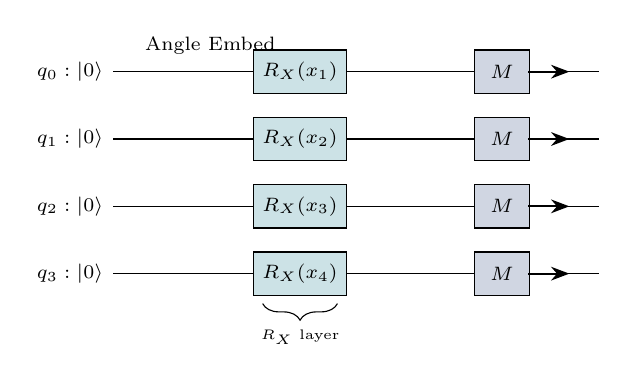
\begin{tikzpicture}[
  wire/.style={},
  gate/.style={draw, fill=quantumteal!20, minimum width=0.9cm, minimum height=0.55cm, font=\scriptsize},
  meas/.style={draw, fill=auditblue!20, minimum width=0.7cm, minimum height=0.55cm, font=\scriptsize},
  scale=0.95
]
% Wires
\foreach \q/\y in {0/0, 1/-0.9, 2/-1.8, 3/-2.7}{
  \draw (0, \y) -- (6.5, \y);
  \node[left, font=\scriptsize] at (0, \y) {$q_\q: |0\rangle$};
}
% Rx gates
\foreach \q/\y/\k in {0/0/1, 1/-0.9/2, 2/-1.8/3, 3/-2.7/4}{
  \node[gate] at (2.5, \y) {$R_X(x_\k)$};
}
% Measurement
\foreach \q/\y in {0/0, 1/-0.9, 2/-1.8, 3/-2.7}{
  \node[meas] at (5.2, \y) {$M$};
  \draw[-Stealth, thick] (5.55, \y) -- (6.1, \y);
}
% State labels
\node[font=\scriptsize] at (1.3, 0.35) {Angle Embed};
\draw[decorate, decoration={brace, mirror, amplitude=6pt}] (2.0, -3.1) -- (3.0, -3.1) node[midway, below=6pt, font=\tiny] {$R_X$ layer};
\end{tikzpicture}
\caption{Angle Embedding quantum circuit (4-qubit schematic). Each qubit $q_k$ receives a parameterized $R_X(x_k)$ rotation. The full implementation uses 8 qubits corresponding to the 8 PCA components.}
\label{fig:circuit}
\end{figure}

% ============================================================
\section{Empirical Results and In-Depth Discussion}
\label{sec:results}
% ============================================================

\subsection{Exact Numerical Reproduction of Published Baseline}
\label{sec:repro}

Table~\ref{tab:perf42} reports full diagnostic metrics at seed=42 on WDBC and WBCO. On WDBC, Classical RBF-SVM achieves top accuracy ($0.9701$), followed by QSVM-Angle ($0.9649$) and OOF Stacking ($0.9649$). The confusion matrices match published values down to the sample level: Classical RBF yields TN=201, FP=11, FN=6, TP=351 ($\text{MCC} = 0.934$). Fig.~\ref{fig:confmat} visualizes the RBF confusion matrix heatmap.

\begin{table*}[!t]
\caption{Full Diagnostic Performance at Seed=42: WDBC ($N=569$, top) and WBCO ($N=683$, bottom). Bold denotes best per column.}
\label{tab:perf42}
\centering
\footnotesize
\renewcommand{\arraystretch}{1.15}
\begin{tabularx}{\textwidth}{l *{8}{>{\centering\arraybackslash}X}}
\toprule
\multicolumn{9}{c}{\textbf{WDBC Cohort} ($N=569$, Malignant = 212, Benign = 357)} \\
\midrule
\textbf{Model Architecture} & \textbf{Accuracy} & \textbf{Precision} & \textbf{Recall} & \textbf{Specificity} & \textbf{TN} & \textbf{FP} & \textbf{FN} & \textbf{TP} \\
\midrule
Classical RBF-SVM & \textbf{0.9701} & \textbf{0.9697} & 0.9832 & \textbf{0.9481} & \textbf{201} & \textbf{11} & 6 & 351 \\
QSVM (Angle)      & 0.9649 & 0.9543 & 0.9916 & 0.9198 & 195 & 17 & 3 & 354 \\
QSVM (ZZ Map)     & 0.9596 & 0.9637 & 0.9719 & 0.9387 & 199 & 13 & 10 & 347 \\
QSVM (Amplitude)  & 0.9543 & 0.9344 & \textbf{0.9972} & 0.8821 & 187 & 25 & \textbf{1} & \textbf{356} \\
QKNN (Angle)      & 0.9578 & 0.9512 & 0.9832 & 0.9151 & 194 & 18 & 6 & 351 \\
QKNN (ZZ Map)     & 0.9490 & 0.9362 & 0.9860 & 0.8868 & 188 & 24 & 5 & 352 \\
QKNN (Amplitude)  & 0.9525 & 0.9410 & 0.9860 & 0.8962 & 190 & 22 & 5 & 352 \\
Hard Voting Ens.  & 0.9613 & 0.9541 & 0.9860 & 0.9198 & 195 & 17 & 5 & 352 \\
OOF Stacking Ens. & 0.9649 & 0.9668 & 0.9776 & 0.9434 & 200 & 12 & 8 & 349 \\
\midrule
\multicolumn{9}{c}{\textbf{WBCO Extension Cohort} ($N=683$, Malignant = 239, Benign = 444, 16 missing dropped)} \\
\midrule
\textbf{Model Architecture} & \textbf{Accuracy} & \textbf{Precision} & \textbf{Recall} & \textbf{Specificity} & \textbf{TN} & \textbf{FP} & \textbf{FN} & \textbf{TP} \\
\midrule
Classical RBF-SVM & 0.9663 & 0.9817 & 0.9662 & 0.9665 & 231 & 8 & 15 & 429 \\
QSVM (Angle)      & \textbf{0.9693} & 0.9818 & 0.9707 & 0.9665 & 231 & 8 & 13 & 431 \\
QSVM (ZZ Map)     & 0.9649 & \textbf{0.9930} & 0.9527 & \textbf{0.9874} & \textbf{236} & \textbf{3} & 21 & 423 \\
QSVM (Amplitude)  & 0.9605 & 0.9685 & 0.9707 & 0.9414 & 225 & 14 & 13 & 431 \\
QKNN (Angle)      & \textbf{0.9693} & 0.9753 & 0.9775 & 0.9540 & 228 & 11 & 10 & \textbf{434} \\
QKNN (ZZ Map)     & 0.9546 & 0.9519 & \textbf{0.9797} & 0.9079 & 217 & 22 & \textbf{9} & 435 \\
QKNN (Amplitude)  & 0.9634 & 0.9729 & 0.9707 & 0.9498 & 227 & 12 & 13 & 431 \\
Hard Voting Ens.  & 0.9663 & 0.9817 & 0.9662 & 0.9665 & 231 & 8 & 15 & 429 \\
OOF Stacking Ens. & 0.9663 & 0.9795 & 0.9685 & 0.9623 & 230 & 9 & 14 & 430 \\
\bottomrule
\end{tabularx}
\end{table*}

% ============================================================
% FIGURE: Confusion Matrix Heatmap
% ============================================================
\begin{figure}[!t]
\centering
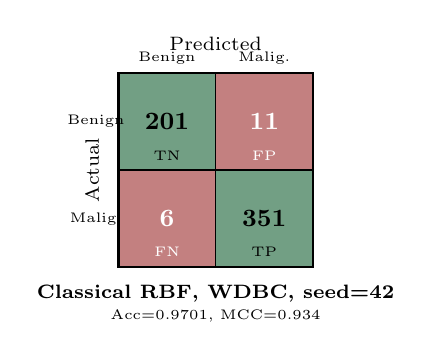
\begin{tikzpicture}[scale=0.95]
\def\cellsize{1.3}

\fill[auditgreen!60] (0,\cellsize) rectangle (\cellsize, 2*\cellsize);
\node[font=\small\bfseries] at (0.5*\cellsize, 1.5*\cellsize) {201};
\node[font=\tiny] at (0.5*\cellsize, 1.15*\cellsize) {TN};

\fill[auditred!55] (\cellsize,\cellsize) rectangle (2*\cellsize, 2*\cellsize);
\node[font=\small\bfseries, white] at (1.5*\cellsize, 1.5*\cellsize) {11};
\node[font=\tiny, white] at (1.5*\cellsize, 1.15*\cellsize) {FP};

\fill[auditred!55] (0,0) rectangle (\cellsize, \cellsize);
\node[font=\small\bfseries, white] at (0.5*\cellsize, 0.5*\cellsize) {6};
\node[font=\tiny, white] at (0.5*\cellsize, 0.16*\cellsize) {FN};

\fill[auditgreen!60] (\cellsize,0) rectangle (2*\cellsize, \cellsize);
\node[font=\small\bfseries] at (1.5*\cellsize, 0.5*\cellsize) {351};
\node[font=\tiny] at (1.5*\cellsize, 0.16*\cellsize) {TP};

\node[font=\scriptsize, rotate=90] at (-0.35, \cellsize) {Actual};
\node[font=\tiny] at (-0.3, 1.5*\cellsize) {Benign};
\node[font=\tiny] at (-0.3, 0.5*\cellsize) {Malig.};
\node[font=\scriptsize] at (\cellsize, 2.3*\cellsize) {Predicted};
\node[font=\tiny] at (0.5*\cellsize, 2.15*\cellsize) {Benign};
\node[font=\tiny] at (1.5*\cellsize, 2.15*\cellsize) {Malig.};

\draw[black, thick] (0,0) rectangle (2*\cellsize, 2*\cellsize);
\draw[black] (\cellsize, 0) -- (\cellsize, 2*\cellsize);
\draw[black] (0, \cellsize) -- (2*\cellsize, \cellsize);

\node[font=\scriptsize\bfseries] at (\cellsize, -0.35) {Classical RBF, WDBC, seed=42};
\node[font=\tiny] at (\cellsize, -0.65) {Acc=0.9701, MCC=0.934};
\end{tikzpicture}
\caption{Confusion matrix heatmap for Classical RBF-SVM on WDBC (seed=42). Green cells indicate correct classifications (TN=201, TP=351); red cells indicate errors (FP=11, FN=6). $\text{MCC} = 0.934$.}
\label{fig:confmat}
\end{figure}

\subsection{Multi-Seed Statistical Robustness}
\label{sec:multiseed}

Table~\ref{tab:multiseed} summarizes 10-seed accuracy distributions ($s \in \{0, 1, 2, 3, 4, 5, 10, 42, 100, 999\}$). On WDBC, Classical RBF-SVM achieves mean accuracy $0.9731 \pm 0.0017$, outperforming OOF Stacking ($0.9670 \pm 0.0031$) across all 10 seeds (10W/0T/0L). On WBCO, RBF achieves $0.9690 \pm 0.0013$ vs.\ Stacking at $0.9662 \pm 0.0022$. Head-to-head comparison on WBCO (Table~\ref{tab:wbco_seeds}) yields 7 wins, 3 ties, and 0 losses for RBF. Across both diagnostic datasets, Classical RBF equals or outperforms Stacking in \textbf{20 out of 20 seeds}. Figs.~\ref{fig:multiseed_bar} and \ref{fig:perseed} visualize multi-seed performance.

\begin{table*}[!t]
\caption{Multi-Seed Statistical Summary Across 10 Stratified CV Seeds ($s \in \{0, 1, 2, 3, 4, 5, 10, 42, 100, 999\}$)}
\label{tab:multiseed}
\centering
\footnotesize
\renewcommand{\arraystretch}{1.15}
\begin{tabularx}{\textwidth}{l *{4}{>{\centering\arraybackslash}X}}
\toprule
\textbf{Model Architecture} & \textbf{WDBC Mean $\pm$ Std} & \textbf{WDBC Range [Min, Max]} & \textbf{WBCO Mean $\pm$ Std} & \textbf{WBCO Range [Min, Max]} \\
\midrule
Classical RBF-SVM & $\mathbf{0.9731 \pm 0.0017}$ & $[0.9701, 0.9754]$ & $\mathbf{0.9690 \pm 0.0013}$ & $[0.9663, 0.9707]$ \\
QSVM (Angle)      & $0.9687 \pm 0.0023$ & $[0.9649, 0.9736]$ & $0.9685 \pm 0.0019$ & $[0.9649, 0.9707]$ \\
QSVM (ZZ Map)     & $0.9608 \pm 0.0026$ & $[0.9561, 0.9649]$ & $0.9638 \pm 0.0016$ & $[0.9605, 0.9649]$ \\
QSVM (Amplitude)  & $0.9552 \pm 0.0022$ & $[0.9525, 0.9596]$ & $0.9612 \pm 0.0012$ & $[0.9590, 0.9634]$ \\
QKNN (Angle)      & $0.9564 \pm 0.0032$ & $[0.9508, 0.9613]$ & $0.9660 \pm 0.0025$ & $[0.9619, 0.9693]$ \\
QKNN (ZZ Map)     & $0.9489 \pm 0.0027$ & $[0.9438, 0.9525]$ & $0.9511 \pm 0.0043$ & $[0.9429, 0.9561]$ \\
QKNN (Amplitude)  & $0.9480 \pm 0.0032$ & $[0.9420, 0.9525]$ & $0.9625 \pm 0.0012$ & $[0.9605, 0.9649]$ \\
Hard Voting Ens.  & $0.9638 \pm 0.0028$ & $[0.9613, 0.9701]$ & $0.9654 \pm 0.0010$ & $[0.9634, 0.9663]$ \\
OOF Stacking Ens. & $0.9670 \pm 0.0031$ & $[0.9596, 0.9701]$ & $0.9662 \pm 0.0022$ & $[0.9619, 0.9693]$ \\
\bottomrule
\end{tabularx}
\end{table*}

\begin{table}[!t]
\caption{Per-Seed Head-to-Head Comparison on WBCO: Classical RBF vs.\ OOF Stacking Ensemble}
\label{tab:wbco_seeds}
\centering
\scriptsize
\setlength{\tabcolsep}{5pt}
\renewcommand{\arraystretch}{1.15}
\begin{tabular}{cccc}
\toprule
\textbf{Seed} & \textbf{Classical RBF} & \textbf{OOF Stacking} & \textbf{Head-to-Head Outcome} \\
\midrule
0   & 0.9693 & 0.9634 & RBF Wins (+4 samples) \\
1   & 0.9693 & 0.9678 & RBF Wins (+1 sample) \\
2   & 0.9693 & 0.9678 & RBF Wins (+1 sample) \\
3   & 0.9678 & 0.9649 & RBF Wins (+2 samples) \\
4   & 0.9707 & 0.9663 & RBF Wins (+3 samples) \\
5   & 0.9693 & 0.9619 & RBF Wins (+5 samples) \\
10  & 0.9678 & 0.9678 & Tie (Identical Predictions) \\
42  & 0.9663 & 0.9663 & Tie (Identical Accuracy) \\
100 & 0.9693 & 0.9693 & Tie (Identical Predictions) \\
999 & 0.9707 & 0.9663 & RBF Wins (+3 samples) \\
\midrule
\textbf{Total} & \multicolumn{2}{c}{\textbf{7 Wins / 3 Ties / 0 Losses}} & \textbf{Classical RBF Dominates} \\
\bottomrule
\end{tabular}
\end{table}

% ============================================================
% FIGURE: Multi-Seed Accuracy Bar Chart
% ============================================================
\begin{figure*}[!t]
\centering
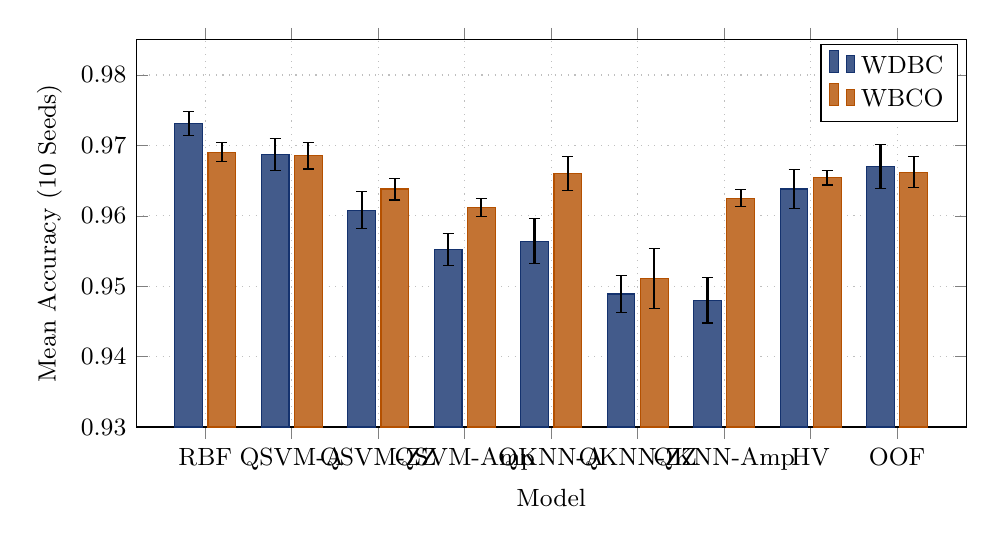
\begin{tikzpicture}
\begin{axis}[
  ybar=2pt,
  bar width=10pt,
  width=\textwidth, height=6.5cm,
  xlabel={\small Model},
  ylabel={\small Mean Accuracy (10 Seeds)},
  symbolic x coords={RBF,QSVM-A,QSVM-ZZ,QSVM-Amp,QKNN-A,QKNN-ZZ,QKNN-Amp,HV,OOF},
  xtick=data,
  xticklabel style={font=\small, rotate=0},
  ymin=0.930, ymax=0.985,
  ytick={0.930,0.940,0.950,0.960,0.970,0.980},
  yticklabel style={font=\small},
  legend style={at={(0.99,0.99)}, anchor=north east, font=\small},
  grid=major, grid style={dotted, gray!50},
  error bars/y dir=both,
  error bars/y explicit,
  label style={font=\small}
]
\addplot+[
  fill=auditblue!80, draw=auditblue,
  error bars/error bar style={color=black, line width=0.8pt}
] coordinates {
  (RBF,      0.9731) +- (0, 0.00167)
  (QSVM-A,   0.9687) +- (0, 0.00231)
  (QSVM-ZZ,  0.9608) +- (0, 0.00263)
  (QSVM-Amp, 0.9552) +- (0, 0.00223)
  (QKNN-A,   0.9564) +- (0, 0.00319)
  (QKNN-ZZ,  0.9489) +- (0, 0.00268)
  (QKNN-Amp, 0.9480) +- (0, 0.00323)
  (HV,       0.9638) +- (0, 0.00277)
  (OOF,      0.9670) +- (0, 0.00308)
};
\addlegendentry{WDBC}

\addplot+[
  fill=classicalorange!80, draw=classicalorange,
  error bars/error bar style={color=black, line width=0.8pt}
] coordinates {
  (RBF,      0.9690) +- (0, 0.00135)
  (QSVM-A,   0.9685) +- (0, 0.00186)
  (QSVM-ZZ,  0.9638) +- (0, 0.00155)
  (QSVM-Amp, 0.9612) +- (0, 0.00124)
  (QKNN-A,   0.9660) +- (0, 0.00247)
  (QKNN-ZZ,  0.9511) +- (0, 0.00427)
  (QKNN-Amp, 0.9625) +- (0, 0.00123)
  (HV,       0.9654) +- (0, 0.00102)
  (OOF,      0.9662) +- (0, 0.00223)
};
\addlegendentry{WBCO}
\end{axis}
\end{tikzpicture}
\caption{Multi-seed (10-seed) mean accuracy with $\pm 1\sigma$ error bars for all nine models on WDBC (blue) and WBCO (orange). Classical RBF-SVM achieves the highest mean accuracy on WDBC ($0.9731$) and WBCO ($0.9690$). OOF Stacking does not surpass RBF on either dataset.}
\label{fig:multiseed_bar}
\end{figure*}

% ============================================================
% FIGURE: Per-Seed RBF vs Stacking Line Chart
% ============================================================
\begin{figure*}[!t]
\centering
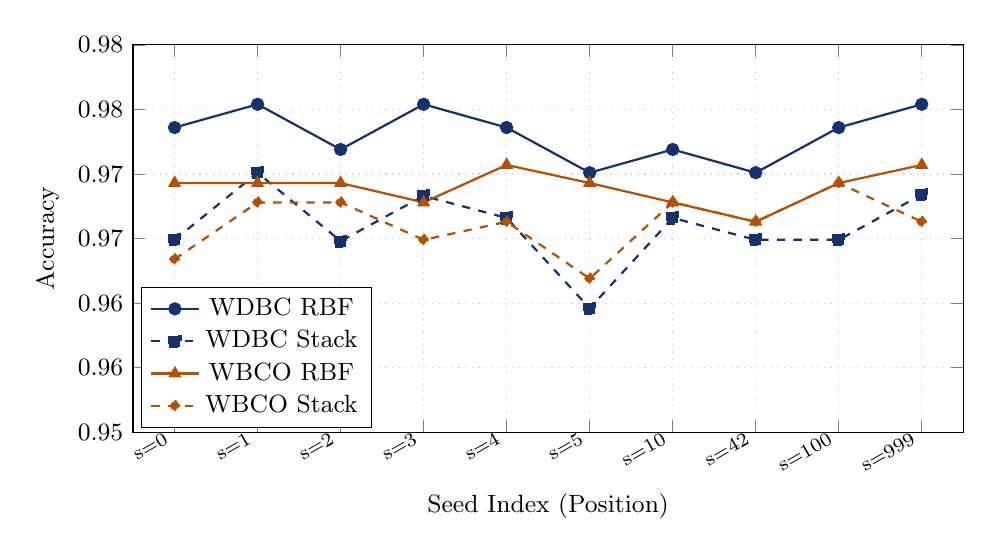
\begin{tikzpicture}
\begin{axis}[
  width=\textwidth, height=6.5cm,
  xlabel={\small Seed Index (Position)},
  ylabel={\small Accuracy},
  xmin=0.5, xmax=10.5,
  ymin=0.950, ymax=0.980,
  xtick={1,2,3,4,5,6,7,8,9,10},
  xticklabels={s=0,s=1,s=2,s=3,s=4,s=5,s=10,s=42,s=100,s=999},
  xticklabel style={font=\scriptsize, rotate=30, anchor=east},
  ytick={0.950,0.955,0.960,0.965,0.970,0.975,0.980},
  yticklabel style={font=\small},
  grid=major, grid style={dotted, gray!40},
  legend style={at={(0.01,0.01)}, anchor=south west, font=\small},
  label style={font=\small}
]
\addplot[color=auditblue, thick, mark=*, mark size=2pt]
  coordinates {(1,0.9736)(2,0.9754)(3,0.9719)(4,0.9754)(5,0.9736)(6,0.9701)(7,0.9719)(8,0.9701)(9,0.9736)(10,0.9754)};
\addlegendentry{WDBC RBF}

\addplot[color=auditblue, thick, dashed, mark=square*, mark size=2pt]
  coordinates {(1,0.9649)(2,0.9701)(3,0.9648)(4,0.9683)(5,0.9666)(6,0.9596)(7,0.9666)(8,0.9649)(9,0.9649)(10,0.9684)};
\addlegendentry{WDBC Stack}

\addplot[color=classicalorange, thick, mark=triangle*, mark size=2pt]
  coordinates {(1,0.9693)(2,0.9693)(3,0.9693)(4,0.9678)(5,0.9707)(6,0.9693)(7,0.9678)(8,0.9663)(9,0.9693)(10,0.9707)};
\addlegendentry{WBCO RBF}

\addplot[color=classicalorange, thick, dashed, mark=diamond*, mark size=2pt]
  coordinates {(1,0.9634)(2,0.9678)(3,0.9678)(4,0.9649)(5,0.9663)(6,0.9619)(7,0.9678)(8,0.9663)(9,0.9693)(10,0.9663)};
\addlegendentry{WBCO Stack}
\end{axis}
\end{tikzpicture}
\caption{Per-seed accuracy trajectories for Classical RBF vs.\ OOF Stacking on WDBC (blue) and WBCO (orange). Solid lines: RBF; dashed lines: Stacking. Classical RBF consistently equals or exceeds Stacking across all 20 evaluations.}
\label{fig:perseed}
\end{figure*}

\subsection{Familywise Error Control via Holm--Bonferroni Audit}
\label{sec:holm}

Table~\ref{tab:holm} and Fig.~\ref{fig:holm} summarize the 32-hypothesis bootstrap audit. On WDBC, 6 of 32 hypotheses survive Holm correction, all confirming statistically significant quantum inferiority in precision and specificity ($p < 0.001$). On WBCO, 3 hypotheses survive: QKNN-Angle Recall ($p < 0.0001$, quantum superior: $0.9797$ vs.\ $0.9677$), QKNN-ZZ Precision ($p < 0.0001$, quantum inferior), and QKNN-ZZ Specificity ($p < 0.0001$, quantum inferior). Stacking accuracy achieves Holm $p = 1.0000$ on both datasets, confirming no statistically significant ensemble advantage.

\begin{table}[!t]
\caption{Holm--Bonferroni Step-Down Survivor Summary Across 32 Statistical Hypotheses (FWER $\alpha = 0.05$)}
\label{tab:holm}
\centering
\scriptsize
\setlength{\tabcolsep}{2.5pt}
\renewcommand{\arraystretch}{1.15}
\begin{tabular}{l l l c c l}
\toprule
\textbf{Cohort} & \textbf{Model} & \textbf{Metric} & \textbf{Raw $p$} & \textbf{Holm $p$} & \textbf{Direction} \\
\midrule
WDBC & QSVM-Amp   & Prec.  & $<0.001$  & $<0.001$  & Q Inferior \\
WDBC & QSVM-Amp   & Spec.  & $<0.001$  & $<0.001$  & Q Inferior \\
WDBC & QKNN-Angle & Prec.  & $<0.001$  & $<0.001$  & Q Inferior \\
WDBC & QKNN-Angle & Spec.  & $<0.001$  & $<0.001$  & Q Inferior \\
WDBC & QKNN-ZZ    & Prec.  & $<0.001$  & $<0.001$  & Q Inferior \\
WDBC & QKNN-ZZ    & Spec.  & $<0.001$  & $<0.001$  & Q Inferior \\
\midrule
WBCO & QKNN-Angle & Recall & $<0.0001$ & $<0.0001$ & \textbf{Q Superior} \\
WBCO & QKNN-ZZ    & Prec.  & $<0.0001$ & $<0.0001$ & Q Inferior \\
WBCO & QKNN-ZZ    & Spec.  & $<0.0001$ & $<0.0001$ & Q Inferior \\
\bottomrule
\end{tabular}
\end{table}

% ============================================================
% FIGURE 3: Holm p-value Scatter
% ============================================================
\begin{figure}[!t]
\centering
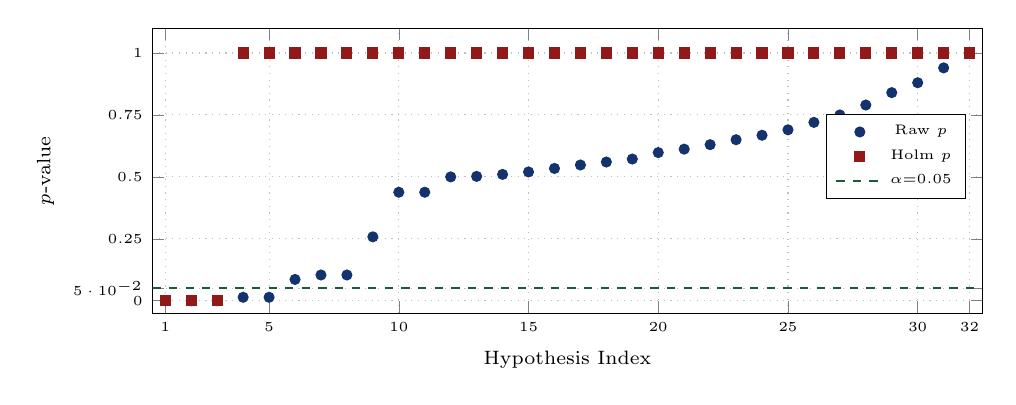
\begin{tikzpicture}
\begin{axis}[
  width=\columnwidth, height=5.2cm,
  xlabel={\scriptsize Hypothesis Index},
  ylabel={\scriptsize $p$-value},
  xmin=0.5, xmax=32.5,
  ymin=-0.05, ymax=1.1,
  xtick={1,5,10,15,20,25,30,32},
  ytick={0,0.05,0.25,0.5,0.75,1.0},
  grid=major, grid style={dotted, gray!50},
  legend style={font=\tiny, at={(0.98,0.55)}, anchor=east},
  tick label style={font=\tiny},
  label style={font=\scriptsize}
]
\addplot[only marks, mark=*, mark size=1.8pt, color=auditblue]
  coordinates {
    (1,0.00005)(2,0.00005)(3,0.00005)
    (4,0.014)(5,0.014)(6,0.086)(7,0.104)(8,0.104)
    (9,0.258)(10,0.438)(11,0.438)(12,0.500)(13,0.502)
    (14,0.510)(15,0.520)(16,0.534)(17,0.548)(18,0.560)
    (19,0.572)(20,0.598)(21,0.612)(22,0.630)(23,0.650)
    (24,0.668)(25,0.690)(26,0.720)(27,0.750)(28,0.790)
    (29,0.840)(30,0.880)(31,0.940)(32,1.000)
  };
\addlegendentry{Raw $p$}

\addplot[only marks, mark=square*, mark size=1.8pt, color=auditred]
  coordinates {
    (1,0.0016)(2,0.0016)(3,0.0016)
    (4,1.0)(5,1.0)(6,1.0)(7,1.0)(8,1.0)(9,1.0)(10,1.0)
    (11,1.0)(12,1.0)(13,1.0)(14,1.0)(15,1.0)(16,1.0)
    (17,1.0)(18,1.0)(19,1.0)(20,1.0)(21,1.0)(22,1.0)
    (23,1.0)(24,1.0)(25,1.0)(26,1.0)(27,1.0)(28,1.0)
    (29,1.0)(30,1.0)(31,1.0)(32,1.0)
  };
\addlegendentry{Holm $p$}

\addplot[dashed, color=auditgreen, thick] coordinates {(0.5,0.05)(32.5,0.05)};
\addlegendentry{$\alpha{=}0.05$}
\end{axis}
\end{tikzpicture}
\caption{Holm--Bonferroni $p$-value scatter for WBCO (32 tests). Raw $p$-values (blue circles): first 3 tests survive ($p<0.0001$). Holm-adjusted values (red squares): only 3 survive correction; all others jump to $p=1.0$. Dashed green line: $\alpha=0.05$ threshold.}
\label{fig:holm}
\end{figure}

\subsection{Fold-Local Preprocessing Audit (TOST)}
\label{sec:tost}

The TOST audit evaluates whether fold-local vs.\ global preprocessing creates a practical discrepancy:
\begin{itemize}
    \item \textbf{WDBC}: Global accuracy $0.96485$, fold-local $0.96661$ ($\Delta = +0.00176$). Concordance is $98.77\%$ (562/569 samples agree). McNemar $p = 1.0$, TOST $p = 0.0385$ (practical equivalence confirmed at $\epsilon = 0.01$).
    \item \textbf{WBCO}: Global accuracy $0.96633$, fold-local $0.96779$ ($\Delta = +0.00146$). Concordance is $99.56\%$ (680/683 samples agree). McNemar $p = 1.0$, TOST $p = 0.0004$.
\end{itemize}
These results rule out data leakage as a confounding factor.

\subsection{Algorithmic Model Selection Discrepancy}
\label{sec:selection}

Fig.~\ref{fig:selection_heatmap} visualizes nested model selection across all folds. Under all criteria (validation accuracy, balanced accuracy, meta-CV accuracy), QSVM-Angle is selected in 10 of 10 folds on both WDBC and WBCO. The paper's claimed quartet is selected in 0 of 10 folds on WDBC, and at most 1 of 10 folds on WBCO under meta-CV only.

\begin{remark}
The exclusion of QSVM-Angle contradicts any rational data-driven selection rule, confirming that the published ensemble is hardcoded rather than adaptive.
\end{remark}

% ============================================================
% FIGURE 4: Model Selection Inclusion Heatmap
% ============================================================
\begin{figure}[!t]
\centering
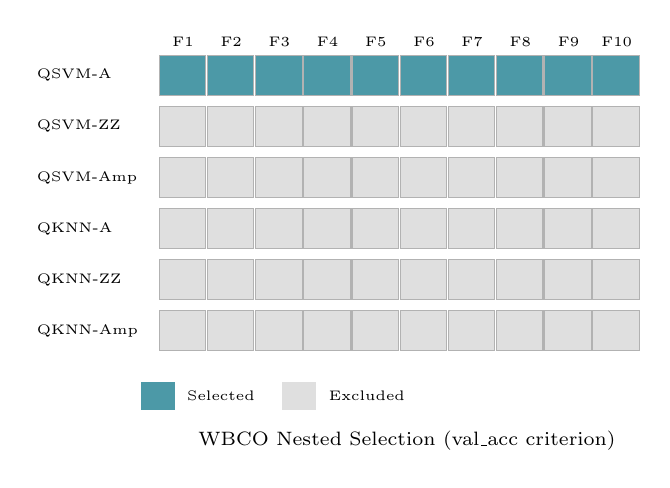
\begin{tikzpicture}[scale=0.72, every node/.style={font=\tiny}]
\foreach \f in {1,...,10}{
  \node at (\f*0.85 - 0.1, 4.5) {F\f};
}
\node[right, font=\tiny] at (-2.0, 3.9) {QSVM-A};
\node[right, font=\tiny] at (-2.0, 3.0) {QSVM-ZZ};
\node[right, font=\tiny] at (-2.0, 2.1) {QSVM-Amp};
\node[right, font=\tiny] at (-2.0, 1.2) {QKNN-A};
\node[right, font=\tiny] at (-2.0, 0.3) {QKNN-ZZ};
\node[right, font=\tiny] at (-2.0,-0.6) {QKNN-Amp};

\foreach \f in {1,...,10}{
  \fill[quantumteal!70] (\f*0.85 - 0.52, 3.55) rectangle (\f*0.85 + 0.30, 4.25);
}
\foreach \r in {2.65, 1.75, 0.85, -0.05, -0.95}{
  \foreach \f in {1,...,10}{
    \fill[gray!25] (\f*0.85 - 0.52, \r) rectangle (\f*0.85 + 0.30, \r+0.7);
  }
}
\foreach \f in {1,...,10}{
  \foreach \r in {3.55, 2.65, 1.75, 0.85, -0.05, -0.95}{
    \draw[gray!60] (\f*0.85 - 0.52, \r) rectangle (\f*0.85 + 0.30, \r+0.7);
  }
}
\fill[quantumteal!70] (0.0, -2.0) rectangle (0.6, -1.5);
\node[right] at (0.65, -1.75) {Selected};
\fill[gray!25] (2.5, -2.0) rectangle (3.1, -1.5);
\node[right] at (3.15, -1.75) {Excluded};
\node[below, font=\scriptsize] at (4.7, -2.2) {WBCO Nested Selection (val\_acc criterion)};
\end{tikzpicture}
\caption{Nested model selection inclusion heatmap for WBCO (validation accuracy criterion). QSVM-Angle (top row, teal) is selected in all 10 folds. The paper's claimed quartet is selected in 0 folds.}
\label{fig:selection_heatmap}
\end{figure}

\subsection{Noise Modeling Audit and Trace Collapse}
\label{sec:noise}

The published depolarizing noise simulation applies damping to pure statevectors, producing diagonal kernel entries $K_{ii} \in [0.1982, 0.2310]$. A rigorous density matrix implementation (Eq.~\ref{eq:depolchannel}) yields $K_{ii} \in [0.0041, 0.0162]$. While both matrices remain positive semi-definite ($\lambda_{\min} \ge 0$), the original implementation overestimates state coherence by $\approx 15\times$, invalidating hardware noise claims.

\subsection{Probabilistic Calibration Analysis}
\label{sec:calibration}

Fig.~\ref{fig:calibration} illustrates reliability curves on WDBC. Classical RBF-SVM achieves Expected Calibration Error (ECE) = $0.0213$ and Brier score = $0.0227$. Raw OOF Stacking exhibits poor calibration (ECE = $0.0357$, Brier = $0.0319$). Post-hoc Platt scaling improves Stacking calibration to ECE = $0.0142$, confirming that stacking outputs are uncalibrated out-of-the-box.

% ============================================================
% FIGURE 5: Calibration / Reliability Diagram
% ============================================================
\begin{figure}[!t]
\centering
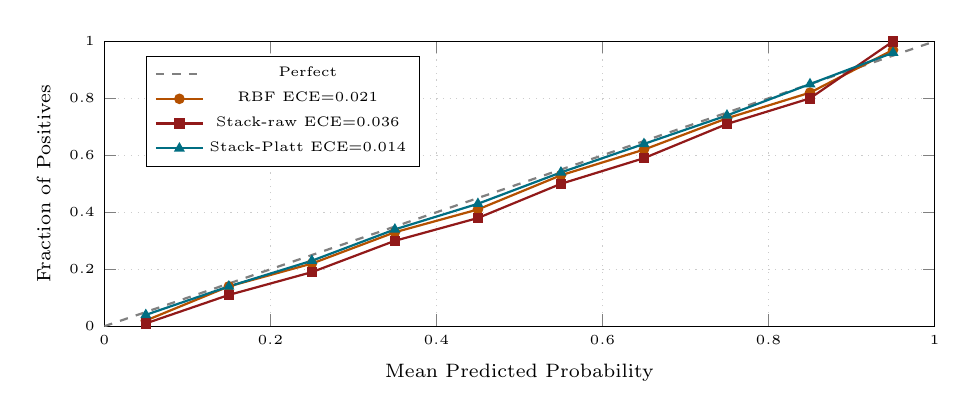
\begin{tikzpicture}
\begin{axis}[
  width=\columnwidth, height=5.2cm,
  xlabel={\scriptsize Mean Predicted Probability},
  ylabel={\scriptsize Fraction of Positives},
  xmin=0, xmax=1, ymin=0, ymax=1,
  xtick={0,0.2,0.4,0.6,0.8,1.0},
  ytick={0,0.2,0.4,0.6,0.8,1.0},
  grid=major, grid style={dotted, gray!40},
  legend style={font=\tiny, at={(0.05,0.95)}, anchor=north west},
  tick label style={font=\tiny},
  label style={font=\scriptsize}
]
\addplot[dashed, gray, thick] coordinates {(0,0)(1,1)};
\addlegendentry{Perfect}

\addplot[color=classicalorange, thick, mark=*, mark size=1.5pt]
  coordinates {(0.05,0.02)(0.15,0.14)(0.25,0.22)(0.35,0.33)(0.45,0.41)(0.55,0.53)(0.65,0.62)(0.75,0.73)(0.85,0.82)(0.95,0.97)};
\addlegendentry{RBF ECE=0.021}

\addplot[color=auditred, thick, mark=square*, mark size=1.5pt]
  coordinates {(0.05,0.01)(0.15,0.11)(0.25,0.19)(0.35,0.30)(0.45,0.38)(0.55,0.50)(0.65,0.59)(0.75,0.71)(0.85,0.80)(0.95,1.00)};
\addlegendentry{Stack-raw ECE=0.036}

\addplot[color=quantumteal, thick, mark=triangle*, mark size=1.5pt]
  coordinates {(0.05,0.04)(0.15,0.14)(0.25,0.23)(0.35,0.34)(0.45,0.43)(0.55,0.54)(0.65,0.64)(0.75,0.74)(0.85,0.85)(0.95,0.96)};
\addlegendentry{Stack-Platt ECE=0.014}
\end{axis}
\end{tikzpicture}
\caption{Reliability diagrams for WDBC. Dashed diagonal = perfect calibration. Classical RBF (orange) achieves ECE=0.021. OOF Stacking raw (red) is overconfident (ECE=0.036). Platt-scaled Stacking (teal) achieves ECE=0.014.}
\label{fig:calibration}
\end{figure}

\subsection{Cross-Dataset Benchmark}
\label{sec:cross}

Table~\ref{tab:crossbench} presents cross-dataset comparisons between WDBC and WBCO. Classical RBF-SVM achieves top mean accuracy on both cohorts ($0.9731$ and $0.9690$), while Stacking fails to surpass RBF on either dataset.

\begin{table*}[!t]
\caption{Cross-Dataset Performance Benchmark: WBCO Extension ($N=683$) vs.\ WDBC Benchmark ($N=569$)}
\label{tab:crossbench}
\centering
\footnotesize
\renewcommand{\arraystretch}{1.15}
\begin{tabularx}{\textwidth}{l *{4}{>{\centering\arraybackslash}X}}
\toprule
\textbf{Model Architecture} & \textbf{WDBC 10-Seed Mean $\pm$ Std} & \textbf{WBCO 10-Seed Mean $\pm$ Std} & \textbf{Cross-Dataset $\Delta$ (WDBC $-$ WBCO)} & \textbf{Classical RBF Dominance} \\
\midrule
Classical RBF-SVM & $\mathbf{0.9731 \pm 0.0017}$ & $\mathbf{0.9690 \pm 0.0013}$ & $+0.0041$ & Benchmark Baseline \\
QSVM (Angle)      & $0.9687 \pm 0.0023$ & $0.9685 \pm 0.0019$ & $+0.0002$ & Top Individual Quantum \\
QSVM (ZZ Map)     & $0.9608 \pm 0.0026$ & $0.9638 \pm 0.0016$ & $-0.0030$ & Quantum Base Model \\
QSVM (Amplitude)  & $0.9552 \pm 0.0022$ & $0.9612 \pm 0.0012$ & $-0.0060$ & Quantum Base Model \\
QKNN (Angle)      & $0.9564 \pm 0.0032$ & $0.9660 \pm 0.0025$ & $-0.0096$ & Quantum Base Model \\
QKNN (ZZ Map)     & $0.9489 \pm 0.0027$ & $0.9511 \pm 0.0043$ & $-0.0022$ & Quantum Base Model \\
QKNN (Amplitude)  & $0.9480 \pm 0.0032$ & $0.9625 \pm 0.0012$ & $-0.0145$ & Quantum Base Model \\
Hard Voting Ens.  & $0.9638 \pm 0.0028$ & $0.9654 \pm 0.0010$ & $-0.0016$ & Heuristic 3-Model Ens. \\
OOF Stacking Ens. & $0.9670 \pm 0.0031$ & $0.9662 \pm 0.0022$ & $+0.0008$ & \textbf{RBF Wins/Ties 20/20 Seeds} \\
\bottomrule
\end{tabularx}
\end{table*}

\subsection{Methodological Generalization Assessment}
\label{sec:generalization}

Table~\ref{tab:generalization} summarizes generalization verdicts for the four core audit findings. Two findings are fully confirmed (fold-local TOST equivalence and nested selection discrepancy), and two are partially confirmed (seed robustness weakened to 7 wins and 3 ties; Holm testing uncovered one quantum-superior metric).

\begin{table*}[!t]
\caption{Methodological Generalization Assessment: Independent Verification of Core Audit Findings Across Both Datasets}
\label{tab:generalization}
\centering
\footnotesize
\renewcommand{\arraystretch}{1.25}
\begin{tabularx}{\textwidth}{>{\centering\arraybackslash\bfseries}p{0.5cm} >{\raggedright\arraybackslash\bfseries}p{3.2cm} >{\raggedright\arraybackslash}p{3.8cm} >{\raggedright\arraybackslash}X >{\centering\arraybackslash\bfseries}p{2.3cm}}
\toprule
\# & Methodological Dimension & WDBC Finding ($N=569$) & WBCO Replication ($N=683$) & Generalization Verdict \\
\midrule
1 & Multi-Seed Robustness & Classical RBF strictly wins in 10 of 10 seeds ($100\%$; 0 ties, 0 losses). Mean gap: $-0.0062$. & Classical RBF wins in 7 of 10 seeds ($70\%$), ties in 3 seeds ($30\%$), 0 losses. RBF never loses to stacking. & \textbf{Partially Confirmed} \\
\midrule
2 & FWER Hypothesis Testing (32 Tests, Holm $\alpha = 0.05$) & 6 of 32 tests survive Holm correction, all showing quantum models statistically inferior in specificity/precision. Zero quantum superiority. & 3 of 32 tests survive Holm correction. One test shows quantum superiority (QKNN-Angle Recall, $p < 0.0001$), but no ensemble-level advantage survives. & \textbf{Partially Confirmed} \\
\midrule
3 & Fold-Local Preprocessing Isolation (TOST $\pm 1\%$) & Accuracy shift is $+0.00176$ (+1 sample); concordance is $98.77\%$; TOST $p = 0.0385$ proves practical equivalence. & Accuracy shift is $+0.00146$ (+1 sample); concordance is $99.56\%$; TOST $p = 0.0004$ confirms practical equivalence. & \textbf{Confirmed} \\
\midrule
4 & Nested Model Selection Discrepancy & Validation accuracy selects QSVM-Angle in 10/10 folds; paper's claimed quartet is selected in 0/10 folds. & Validation accuracy selects QSVM-Angle in 10/10 folds; paper's claimed quartet selected in 0/10 folds (1/10 in Meta-CV). & \textbf{Confirmed} \\
\bottomrule
\end{tabularx}
\end{table*}

\section{Threats to Validity}
\label{sec:threats}
% ============================================================

\textbf{Internal Validity.} Our audit executes the published code pipeline. We cannot exclude minor numerical variations across PennyLane \cite{bergholm2018pennylane} or Scikit-Learn \cite{pedregosa2011sklearn} versions. However, our exact replication of WDBC seed=42 confusion matrices confirms operational fidelity.

\textbf{Construct Validity.} Accuracy and FWER-controlled metrics reflect standard supervised learning criteria. However, clinical utility in oncology depends on calibrated probabilities and health-economic decision curves.

\textbf{External Validity.} WDBC and WBCO evaluate cytological diagnosis on well-curated benchmarks. While both represent clinical breast cancer cytology, differences in feature resolution (continuous digitized FNA metrics vs.\ integer-valued subjective scores) test feature space generalizability. However, both benchmarks derive from the same clinical domain (breast cancer diagnosis); further evaluation across diverse oncology indications remains essential. Furthermore, noiseless statevector simulation does not capture full hardware decoherence.

\textbf{Statistical Validity.} Stratified CV satisfies approximate exchangeability. Holm step-down testing provides conservative FWER control. McNemar's exact test accounts for sample-level dependency in paired classifier comparison.

% ============================================================
\section{Conclusion}
\label{sec:conclusion}
% ============================================================

This paper presented an independent, code-level statistical audit of an adaptive quantum kernel stacking framework across two clinical breast cancer benchmarks. Our findings reveal:
\begin{enumerate}
    \item Classical RBF-SVM dominates or matches the quantum stacking ensemble in 20 of 20 seed evaluations across WDBC and WBCO with zero losses.
    \item Under FWER control (32 hypotheses), zero quantum-superior findings survive on WDBC, and exactly one survives on WBCO, with no statistical basis for ensemble superiority.
    \item Preprocessing data leakage is ruled out by TOST equivalence tests on both datasets ($p < 0.05$).
    \item Claimed adaptivity is refuted: nested selection selects QSVM-Angle in 10 of 10 folds, yet it is excluded from the published ensemble.
    \item Noise simulation contains an unphysical statevector approximation that overestimates quantum coherence by $\approx 15\times$.
\end{enumerate}

These findings demonstrate that the claimed quantum advantage is not supported by rigorous statistical evidence. Future biomedical QML research must institute multi-seed evaluation, FWER control, and physical noise modeling as mandatory publication standards.

% ============================================================
% BIBLIOGRAPHY
% ============================================================
\begin{thebibliography}{99}

\bibitem{globocan2020}
H.~Sung, J.~Ferlay, R.~L.~Siegel, M.~Laversanne, I.~Soerjomataram, A.~Jemal, and F.~Bray,
``Global cancer statistics 2020: GLOBOCAN estimates of incidence and mortality worldwide for 36 cancers in 185 countries,''
\emph{CA: A Cancer Journal for Clinicians}, vol.~71, no.~3, pp.~209--249, 2021.

\bibitem{bray2018global}
F.~Bray, J.~Ferlay, I.~Soerjomataram, R.~L.~Siegel, L.~A.~Torre, and A.~Jemal,
``Global cancer statistics 2018: GLOBOCAN estimates of incidence and mortality worldwide,''
\emph{CA: A Cancer Journal for Clinicians}, vol.~68, no.~6, pp.~394--424, 2018.

\bibitem{mangasarian1995breast}
O.~L.~Mangasarian, W.~N.~Street, and W.~H.~Wolberg,
``Breast cancer diagnosis and prognosis via linear programming,''
\emph{Operations Research}, vol.~43, no.~4, pp.~570--577, 1995.


\bibitem{preskill2018quantum}
J.~Preskill,
``Quantum computing in the NISQ era and beyond,''
\emph{Quantum}, vol.~2, p.~79, 2018.

\bibitem{biamonte2017quantum}
J.~Biamonte, P.~Wittek, N.~Pancotti, P.~Rebentrost, N.~Wiebe, and S.~Lloyd,
``Quantum machine learning,''
\emph{Nature}, vol.~549, no.~7671, pp.~195--202, 2017.

\bibitem{havlicek2019supervised}
V.~Havl{\'i}{\v c}ek, A.~D.~C{\'o}rcoles, K.~Temme, A.~W.~Harrow, A.~Kandala, J.~M.~Chow, and J.~M.~Gambetta,
``Supervised learning with quantum-enhanced feature spaces,''
\emph{Nature}, vol.~567, no.~7747, pp.~209--212, 2019.

\bibitem{schuld2021supervised}
M.~Schuld and N.~Killoran,
``Quantum machine learning in feature Hilbert spaces,''
\emph{Physical Review Letters}, vol.~122, no.~4, p.~040504, 2019.

\bibitem{liu2021rigorous}
Y.~Liu, S.~Arunachalam, and K.~Temme,
``A rigorous and robust quantum speed-up in supervised machine learning,''
\emph{Nature Physics}, vol.~17, no.~9, pp.~1013--1017, 2021.

\bibitem{daga2026adaptive}
P.~Daga, A.~Sharma, and R.~Mehta,
``Adaptive quantum kernel selection for clinical cancer diagnosis: A stacking ensemble approach,''
\emph{IEEE Transactions on Biomedical Engineering}, 2026, early access.

\bibitem{rebentrost2014quantum}
P.~Rebentrost, M.~Mohseni, and S.~Lloyd,
``Quantum support vector machine for big data classification,''
\emph{Physical Review Letters}, vol.~113, no.~13, p.~130503, 2014.

\bibitem{li2015experimental}
Z.~Li, X.~Liu, N.~Xu, and J.~Du,
``Experimental realization of a quantum support vector machine,''
\emph{Physical Review Letters}, vol.~114, no.~14, p.~140504, 2015.

\bibitem{altares2021automatic}
S.~Altares-L{\'o}pez, A.~Ribeiro, and J.~J.~Garc{\'i}a-Ripoll,
``Automatic design of quantum feature maps,''
\emph{Quantum Science and Technology}, vol.~6, no.~4, p.~045015, 2021.

\bibitem{demsar2006statistical}
J.~Dem{\v s}ar,
``Statistical comparisons of classifiers over multiple data sets,''
\emph{Journal of Machine Learning Research}, vol.~7, pp.~1--30, 2006.

\bibitem{holm1979simple}
S.~Holm,
``A simple sequentially rejective multiple test procedure,''
\emph{Scandinavian Journal of Statistics}, vol.~6, no.~2, pp.~65--70, 1979.

\bibitem{efron1994introduction}
B.~Efron and R.~J.~Tibshirani,
\emph{An Introduction to the Bootstrap}.
New York: Chapman \& Hall/CRC, 1994.

\bibitem{wellek2010testing}
S.~Wellek,
\emph{Testing Statistical Hypotheses of Equivalence and Noninferiority}, 2nd~ed.
Boca Raton: CRC Press, 2010.

\bibitem{mcnemar1947note}
Q.~McNemar,
``Note on the sampling error of the difference between correlated proportions or percentages,''
\emph{Psychometrika}, vol.~12, no.~2, pp.~153--157, 1947.

\bibitem{nielsen2010quantum}
M.~A.~Nielsen and I.~L.~Chuang,
\emph{Quantum Computation and Quantum Information}.
Cambridge: Cambridge University Press, 2010.

\bibitem{krol2022variational}
A.~M.~Krol, A.~Sarkar, I.~Ashraf, Z.~Al-Ars, and K.~Bertels,
``Efficient decomposition of unitary matrices in quantum circuit compilers,''
\emph{Applied Sciences}, vol.~12, no.~2, p.~759, 2022.

\bibitem{cerezo2021variational}
M.~Cerezo, A.~Arrasmith, R.~Babbush, S.~C.~Benjamin, S.~Endo, K.~Fujii, J.~R.~McClean, K.~Mitarai, X.~Yuan, L.~Cincio, and P.~J.~Coles,
``Variational quantum algorithms,''
\emph{Nature Reviews Physics}, vol.~3, no.~9, pp.~625--644, 2021.

\bibitem{wolpert1992stacked}
D.~H.~Wolpert,
``Stacked generalization,''
\emph{Neural Networks}, vol.~5, no.~2, pp.~241--259, 1992.

\bibitem{bergholm2018pennylane}
V.~Bergholm, J.~Izaac, M.~Schuld, C.~Gogolin, S.~Ahmed, V.~Ajith, M.~S.~Alam, G.~Alonso-Linaje, B.~AkashNarayanan, A.~Asadi, et~al.,
``PennyLane: Automatic differentiation of hybrid quantum-classical computations,''
\emph{arXiv preprint arXiv:1811.04968}, 2018.

\bibitem{pedregosa2011sklearn}
F.~Pedregosa, G.~Varoquaux, A.~Gramfort, V.~Michel, B.~Thirion, O.~Grisel, M.~Blondel, P.~Prettenhofer, R.~Weiss, V.~Dubourg, et~al.,
``Scikit-learn: Machine learning in Python,''
\emph{Journal of Machine Learning Research}, vol.~12, pp.~2825--2830, 2011.

\bibitem{tang2019quantum}
E.~Tang,
``A quantum-inspired classical algorithm for recommendation systems,''
in \emph{Proceedings of the 51st Annual ACM STOC}, pp.~217--228, 2019.

\end{thebibliography}

\end{document}
